\section{Architecture} \label{sec:architecture}
In simple terms, a BF machine consists of an array of memory-cells, together with a pointer pointing to one of these cells. The pointer can move along the array while modifying its contents one step at a time. An example of this representation in some intermediate state is shown in Figure \ref{fig:simplerepresentation}. Consider the BF program ``\texttt{>>>>>+.}'', applied to the initial conditions shown in the example. The pointer would take 5 steps to the right, landing on cell 9 which contains the number 41. It will then increment and output this value, displaying 42 on the screen (assuming a screen of some sort is used as the output device and it is displaying numbers directly rather than interpreting them as ASCII).

\begin{figure}[H]
  \centering
  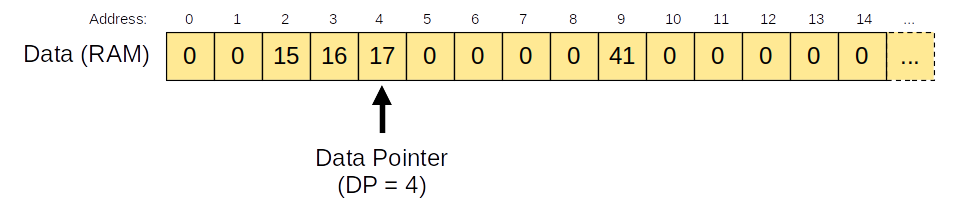
\includegraphics[width=0.9\textwidth]{img/simple_representation}
  \caption{Example state of a BF machine.}
  \label{fig:simplerepresentation}
\end{figure}


In practice, a physical implementation of a machine like this needs many more components in addition to the RAM and Data Pointer in order to perform all the necessary operations. This chapter will list the modules that comprise the BF processor and give an overview of the way these modules function and communicate. The actual implementation on the logic/hardware level is described in section \ref{sec:implementation}.

\subsection{Overview} \label{sec:architecture:overview}
The processor consists of three basic building blocks: registers, memory and a control unit. The ALU is missing from this list because the only operations that it needs to perform are addition and subtraction of the value 1, which can be done directly at the register-level when using up/down binary counters like the 74LS193 integrated circuit. The program (a sequence of BF instructions) is stored into Read Only Memory (ROM), whereas the data is stored in Random Access Memory (RAM). Instructions (4-bits) are loaded from ROM into the instruction register (I), together with some flags that encode the state of the machine. Depending on the state and current instruction, the Control Unit sets the appropriate control signals for each of the modules in order for the system to perform the next computation. Figure \ref{fig:architecture} shows how each of the modules is communicating with other modules. In the sections below, each of these connections will be clarified further.

\begin{figure}[H]
  \centering
  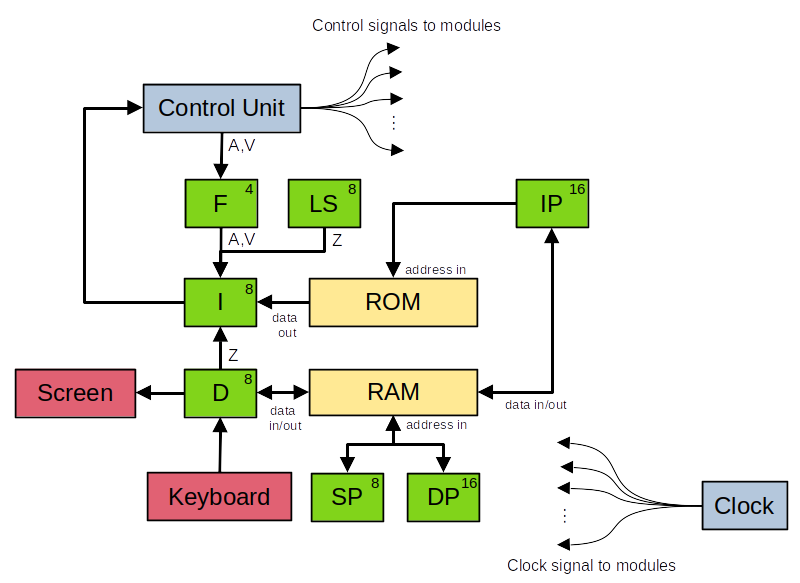
\includegraphics[width=0.9\textwidth]{img/bfcpu_architecture}
  \caption{Connections between modules in the BF processor.}
  \label{fig:architecture}
\end{figure}

\subsection{Instruction Pointer Register (IP)} \label{sec:architecture:ipreg}
The instruction pointer is a 16-bit value, kept in the IP register, which keeps track of the current instruction that is being executed. It points to a certain address in ROM (which stores the program) and is usually incremented after each instruction has finished executing, in order to move to the next instruction. However, when the processor encounters the \texttt{[}-instruction (and the loop is entered), it needs to store the current value of the IP somewhere in order to be able to jump back to this location. The value is therefore stored on the stack (the first part of RAM). When the matching \texttt{]}-instruction is encountered, this value is loaded back into the IP instead of simply incrementing the previous value. This has the effect of jumping back in the program, which is how loops are implemented in BF.

\subsection{Stack Pointer (SP)} \label{sec:architecture:spreg}
The stack is the first part of RAM (addresses 0x0000 - 0x00ff) which is reserved to keep track of addresses that might need to be jumped to. The stack-pointer (SP) is incremented whenever a new value is stored on the stack and decremented whenever a value is popped off the stack. In this implementation, the SP is an 8-bit value, which means that at most 256 different values can be stored onto the stack before it the SP overflows (wraps around back to 0) and starts overwriting previous values. This would happen if a BF program was loaded that has more than 256 nested \texttt{[]}-pairs. Although possible, it is very unlikely to happen for the simple programs we intend to run.

\subsection{Instruction Register (I)} \label{sec:architecture:ireg}
The instruction register is an 8-bit register that stores the current instruction, which was loaded from ROM according to the IP value. The BF-instruction itself is only 4 bits wide, which leaves another 4 bits for encoding the state of the machine, using flags. There are 4 flags that determine the state of the machine:
\begin{itemize}
\item Z(D): the zero-flag set by the D-register, indicating that there is currently a 0 stored in this register;
\item Z(LS): the zero-flag set by the LS-register (see \ref{sec:architecture:loopskip});
\item A: the address-changed-flag, set by the control-unit, indicating that the previous instruction has changed the value of the data-pointer. When this flag is set, the value in the D-register does no longer correspond to the cell pointed to by the data-pointer;
\item V: the value-changed-flag, set by the control-unit, indicating that the previous instruction has altered the value in the D-register. When this flag is set, the value in RAM is outdated and needs to be updated before moving the pointer to a different cell.
\end{itemize}

\subsection{Data Register (D) and Data Pointer Register (DP)} \label{sec:architecture:danddp}
The data-pointer corresponds to the pointer as specified in the BF-language. It points to some value in memory beyond the stack ($\ge$ 0x0100) and can be either incremented (moved right) or decremented (moved left) using the \texttt{>} and \texttt{<} instructions. Whenever the value pointed to by DP is modified by \texttt{+} or \texttt{-}, it is loaded into the D-register, where it can be modified before being stored back into RAM. This happens in conjunction with the flag-register, which dictates whether or not synchronization has to take place between RAM and D (see also section \ref{sec:architecture:flags}).

\subsection{Flags and the Flag Register (F)} \label{sec:architecture:flags}
\subsubsection{A and V}
A naive and fail-safe way of synchronizing the contents of RAM with the contents of the D-register, is to perform the following sequence on each \texttt{+} or \texttt{-} instruction:
\begin{enumerate}
\item Load the current value (pointed to by DP) into D;
\item Modify the value;
\item Write the value back into RAM.
\end{enumerate}
However, it is very common to have sequences of many repeating \texttt{+}'s or \texttt{-}'s and it would be a waste to keep writing the contents of D back to RAM, only to read them back into D during the very next instruction. This is why the Control Unit sets a flag whenever either the value of the DP has changed (A, the address-changed-flag) or the value in the D-register has changed (V, the value-changed-flag). Depending on the state of these flags, the Control Unit can determine whether it has to synchronize the RAM with the D-register, or not (yet). The Control Unit buffers these flags in the flag-register (F), which is loaded into the instruction register (I) together with the next instruction from ROM.

\subsubsection{Z(D) and Z(LS)}
In addition to the A and V flags, there are two flags which are not buffered in F, but can be directly loaded into I: the zero-flags (Z) from the data-register and loop-skip-register (see section \ref{sec:architecture:loopskip}). These flags are both used in the context of conditional jumps:
\begin{itemize}
\item Z(D) : When encountering either an opening \texttt{[}, the flag indicates whether or not to enter or skip the loop. On a closing \texttt{]}, the flag indicates whether to loop back or exit from the loop.
\item Z(LS) : The zero-flag from the loop-skip register indicates whether or not we are currently in the process of skipping an entire piece of code. This happens when the current value is 0 when encountering an opening \texttt{[}. In this case, execution must resume after the matching closing \texttt{]}. Only when the LS has its zero-flag set, should the current instruction actually be executed.
\end{itemize}

\subsection{Loop Skip Register (LS)} \label{sec:architecture:loopskip}
The Loop Skip (LS) register is a counter that indicates whether or not we're in the process of sckipping a loop. In BF, a loop (\texttt{[}) is only entered when the value currently pointed to is nonzero. In the case that it is zero, execution resumes beyond its matching \texttt{]}. When it is determined (by the Control Unit) that a loop must be skipped (based on the zero-flag set by the D-register), the LS register is incremented from 0 to 1. Subsequent instructions are then skipped until either another (nested) loop opening \texttt{[} or a closing \texttt{]} is encountered. On the former, the LS is incremented again while on the latter the LS is decremented. This has the effect that the LS becomes 0 again after the \texttt{]} that matches the original \texttt{[} which led to the skip. Normal execution occurs as soon as LS has become 0 again.
    
\subsection{Control Unit} \label{sec:architecture:controlunit}
Each of the aforementioned components/modules has one or more control inputs that determine what happens on the next clock cycle. For example, some register-modules can be told to either load a value from their input, increment or decrement the currently stored value, or do nothing at all. It is the Control Unit (CU) that supplies the appropriate control signals to each of the modules before the next clock pulse occurs. The implementation details of how this is done in hardware are discussed in section \ref{sec:implementation}. The current and next section (\ref{sec:architecture:sequences}), however, will provide an overview of the control signals for each module and the sequences of control signals that are necessary to perform each BF instruction.
\subsubsection{Register Control Signals}
Not all registers (green modules in Figure \ref{fig:architecture}) have the exact same functionality. All of them store a value, but not all are required to count, let alone count in both directions. Table \ref{tab:registers} shows which of the registers are able to perform certain actions. The control signals have been abbrivated according to the following schema:
\begin{itemize}
\item EN: output enable - if this signal is unavailable, its output is either always available or not used at all;
\item LD: load a value from the input;
\item CE: count enable - increment the current value;
\item DEC: if the CE signal is supplied, decrement instead of increment;
\end{itemize}

\begin{table}[H]
  \centering
  \begin{tabular}{c|c|c|c|c|c}
    Register & \#Bits & EN  & LD  & CE  & DEC \\ \hline 
    D        & 8     & Yes & Yes & Yes & Yes \\
    I        & 8     & No  & Yes & No  & No  \\
    DP       & 16    & Yes & No  & Yes & Yes \\ 
    SP       & 8     & Yes & No  & Yes & Yes \\ 
    IP       & 16    & No  & Yes & Yes & No  \\ 
    F        & 4     & No  & Yes & No  & No  \\ 
    LS       & 8     & No  & No  & Yes & Yes \\ 
  \end{tabular}
  \caption{Control signals available to each of the registers.}
  \label{tab:registers}
\end{table}

\subsubsection{Memory (RAM)}
The memory module has an address input and a set of I/O lines which can be used for either storing a new value into memory (input) or outputting the value stored at the current address. It is therefore sufficient to have only two control signals that go into the RAM module:
\begin{itemize}
\item OE: output enable - the value at the current address (supplied on the address lines) will be available at the output;
\item WE: write enable - writes the value at the input to the current address.
\end{itemize}

\subsubsection{Control Unit}
Even though the control unit is setting the control signals for all other modules, it has some control signals that it should be able to set for itself. Depending on the instruction that is being executed, it should write values to the flag register. The control signals to indicate that this is being done are called AE and VE respectively. Moreover, its internal instruction counter should be reset in the final cycle of each instruction. This is indicated with the CR (cycle reset) signal.
\begin{itemize}
\item AE: A-flag enable - outputs a high value into the A-bit of the flag register;
\item VE: V-flag enable - outputs a high value into the V-bit of the flag register.
\item CR: Cycle reset - reset the internal cycle counter to 0 to prepare for the next instruction.
\end{itemize}

\subsubsection{Screen (Output)}
The output module (which is assumed to be a screen) will be directly attached to the data-register and will display whatever is in there, as long as it is told to by a single control signal on the next clock cycle: PRE (print enable).

\subsubsection{Keyboard (Input)}
TBD

\subsection{Control Sequences} \label{sec:architecture:sequences}
Table \ref{tab:microcode} shows the control sequences that are executed per BF instruction. The Control Unit implements this as a lookup table in ROM, where the instruction, flags and cycle counter act as an address into this table and the control signal configuration is stored at this address in ROM. The final microcode instruction of each sequence automatically resets the cycle counter, as a result of which the next instruction will be loaded and executed.

\begin{table}[H] \centerline{
    \centering
    \begin{tabular} {c|cccc|c|llllll}
      Instr      & V & A & Z(LS) & Z(D) & Cycle & \multicolumn{6}{c}{Control Signals}                   \\ \hline
                 &   &   &       &      & 0     & EN(IP) & LD(I)   &         &        &                 \\ \hline
      \texttt{+} &   & 0 & 0     &      & 1     & CE(D)  & VE(CU)  & LD(F)   & CE(IP) & CR(CU)          \\
      
                 &   & 1 & 0     &      & 1     & EN(DP) & LD(D)   & OE(RAM) &        &                 \\ 
                 &   & 1 & 0     &      & 2     & CE(D)  & VE(CU)  & LD(F)   & CE(IP) & CR(CU)          \\
      
                 &   &   & 1     &      & 1     & CE(IP) & CR(CU)  &         &        &                 \\ \hline

      \texttt{-} &   & 0 & 0     &      & 1     & CE(D)  & DEC(D)  & VE(CU)  & LD(F)  & CE(IP) & CR(CU) \\
      
                 &   & 1 & 0     &      & 1     & EN(DP) & LD(D)   & OE(RAM) &        &                 \\ 
                 &   & 1 & 0     &      & 2     & CE(D)  & DEC(D)  & VE(CU)  & LD(F)  & CE(IP) & CR(CU) \\
       
                 &   &   & 1     &      & 1     & CE(IP) & CR(CU)  &         &        &                 \\ \hline

      \texttt{>} & 0 &   & 0     &      & 1     & CE(DP) & AE(CU)  & LD(F)   & CE(IP) & CR(CU)          \\
      
                 & 1 &   & 0     &      & 1     & EN(D)  & EN(DP)  & WE(RAM) &        &                 \\
                 & 1 &   & 0     &      & 2     & CE(DP) & AE(CU)  & LD(F)   & CE(IP) & CR(CU)          \\
      
                 &   &   & 1     &      & 1     & CE(IP) & CR(CU)  &         &        &                 \\ \hline

      \texttt{<} & 0 &   & 0     &      & 1     & CE(DP)  & DEC(DP) & AE(CU)  & LD(F)  & CE(IP) & CR(CU) \\
      
                 & 1 &   & 0     &      & 1     & EN(D)   & EN(DP)  & WE(RAM) &        &                 \\
                 & 1 &   & 0     &      & 2     & CE(DP)  & DEC(DP) & AE(CU)  & LD(F)  & CE(IP) & CR(CU) \\
      
                 &   &   & 1     &      & 1     & CE(IP)  & CR(CU)  &         &        &                 \\ \hline

      \texttt{[} &   & 0 & 0     & 1    & 1     & CE(LS)  & CE(IP) & CR(CU)                              \\
        
                 &   & 0 & 0     & 0    & 1     & CE(SP)                                                \\
                 &   & 0 & 0     & 0    & 2     & WE(RAM) & EN(SP) & EN(IP) \\
                 &   & 0 & 0     & 0    & 3     & CE(IP)  & CR(CU) \\
        
                 &   & 1 & 0     &      & 1     & EN(DP)  & LD(D) & OE(RAM)  \\
                 &   & 1 & 0     &      & 2     & EN(IP)  & LD(I) \\
                 &   & 1 & 0     & 1    & 3     & CE(LS)  & CE(IP) & CR(CU) \\
                 &   & 1 & 0     & 0    & 3     & CE(SP) \\
                 &   & 1 & 0     & 0    & 4     & WE(RAM) & EN(SP) & EN(IP) \\
                 &   & 1 & 0     & 0    & 5     & LD(F) & CE(IP) & CR(CU) \\
      
    \end{tabular}
  }
  \caption{Control signals for each of the BF instructions}
  \label{tab:microcode}
\end{table}
